\documentclass[journal]{IEEEtran}

\usepackage{amsmath,amssymb,amsthm}
\usepackage{graphicx}
\usepackage{booktabs}
\usepackage{xcolor}
\usepackage[hidelinks]{hyperref}
\usepackage{cite}

\newtheorem{theorem}{Theorem}
\newtheorem{lemma}{Lemma}
\newtheorem{corollary}{Corollary}
\newtheorem{definition}{Definition}
\theoremstyle{remark}
\newtheorem{remark}{Remark}
\newcommand{\etaC}{\eta_{\mathrm{C}}}
\newcommand{\todo}[1]{\textcolor{red}{[TODO: #1]}}

\begin{document}

\title{Ratio Objectives Hide the Pareto Front from Weighted-Sum Decomposition: Theory, Diagnostics,
and a Quantum Heat Engine Case Study}

\author{Hugo~Campos%
\thanks{H. Campos is with the Universidad T\'ecnica Federico Santa Mar\'ia, Valpara\'iso, Chile.}}

\markboth{Draft}{Campos: Ratio objectives and weighted-sum decomposition}

\maketitle

\begin{abstract}
Weighted-sum scalarization reaches only the supported part of a Pareto front, so its success depends
on the front's geometry. In real-world problems that geometry is not fixed by the solutions alone:
it depends on which of several equivalent objectives the modeler writes down. We study a structure
common in engineering, where one objective is a \emph{ratio} (an efficiency or yield) and a cost
scales in proportion to an \emph{extensive} output at fixed ratio. We prove that such
product-structured fronts are saddle surfaces, with no supported interior point, and that replacing
the ratio by an extensive cost turns the same set of solutions into the graph of a perspective
function, which is convex exactly when a one-dimensional profile is convex. The convex case is
degenerate along rays, which makes weighted-sum optima non-unique. We propose two diagnostics: a
linear-programming support test and a hypervolume ceiling that splits the loss of weighted-sum
methods into a reachability part and a distribution part. A finite-time quantum Otto engine, whose
Pareto front saturates a thermodynamic uncertainty relation, realizes the structure exactly. With
efficiency as an objective, 91\% of its front is unsupported and six of seven multi-objective
evolutionary algorithms exceed the hypervolume ceiling of any weighted-sum method; with entropy
production, the ceiling coincides with the reference front and the weighted-sum loss is due only to
the degeneracy. A 17-variable variant that breaks the structure has a nearly convex front.
\end{abstract}

\begin{IEEEkeywords}
Decomposition-based multi-objective optimization, weighted sum, Tchebycheff, Pareto front shape,
supported solutions, real-world benchmark, quantum heat engines.
\end{IEEEkeywords}

%=====================================================================
\section{Introduction}
%=====================================================================

\IEEEPARstart{D}{ecomposition}-based multi-objective evolutionary algorithms (MOEAs) turn a
multi-objective problem into a set of scalar subproblems~\cite{ZhangLi2007,Trivedi2017}. The
weighted sum is the simplest scalarizing function, and in many application fields it is still the
default way to trace a front: practitioners define a figure of merit that adds the normalized
objectives with weights and sweep the weights. A classical limitation is that a weighted sum can
only reach the \emph{supported} part of the front, i.e., the points on its convex
hull~\cite{DasDennis1997,Ehrgott2005,Marler2004}. The performance of decomposition-based MOEAs is
known to depend strongly on the front shape~\cite{Ishibuchi2017}.

Front shape is usually treated as a property of the problem. In real-world problems, however, the
modeler often has a choice between objectives that describe the same trade-off. An engine can be
judged by its efficiency or by the entropy it produces; a process by its yield or by its waste; a
plant by its specific cost or its total cost. At fixed output, the two members of each pair are
monotonically related, so they are commonly treated as interchangeable. For dominance-based
algorithms the choice is often immaterial. For weighted-sum scalarization it is not, because the
relation between the two objectives is nonlinear and couples them with the output, and such a
change of coordinates can turn a convex front into a nonconvex one.

This paper characterizes when that happens for a structure that is common in engineering and
physics. We call an objective a \emph{ratio} if it is output per unit input (efficiency, yield), and
\emph{extensive} if it scales with the size of the operation (power, total cost, waste). The
structure we study arises when a third objective, typically a cost or a variability, is proportional
to the extensive output at fixed ratio. Our contributions are:
\begin{enumerate}
\item \emph{Theory} (Sec.~\ref{sec:theory}). Product-structured fronts written with a ratio
objective are saddle surfaces with no supported interior point (Theorem~\ref{thm:saddle}). Rewritten
with an extensive objective, the same solutions form the graph of a perspective function, which is
convex if and only if a one-dimensional profile is convex (Theorem~\ref{thm:perspective}); the convex
case is degenerate along rays (Corollary~\ref{cor:degenerate}). Lower-dimensional (degenerate) fronts
escape the first result.
\item \emph{Diagnostics} (Sec.~\ref{sec:diagnostics}). A linear-programming support test, a
hypervolume (HV) ceiling of all weighted-sum methods that decomposes their HV loss into reachability
and distribution, and a multiplicative $\varepsilon$ loss of the best reachable solution.
\item \emph{A real-world case study} (Sec.~\ref{sec:case}). A finite-time quantum Otto engine whose
Pareto front saturates a thermodynamic uncertainty relation and therefore realizes the product
structure exactly, in two equivalent formulations. Its evaluation is exact and cheap, and its front
shape is analytically known, which makes it a useful benchmark. A 17-variable piecewise-control
variant breaks the structure.
\item \emph{An empirical study} (Secs.~\ref{sec:setup}--\ref{sec:results}) of seven MOEAs, with 30
runs each on both models and both formulations, that confirms the predictions and separates the two
mechanisms by which weighted-sum decomposition loses quality.
\end{enumerate}

Transformations that convexify a front are not new: separable power transformations of the
objectives can make a weighted sum reach nonconvex parts~\cite{Li1996}. The reformulations studied
here are different in kind: they are physically meaningful, they mix two objectives, and they can
convexify or deconvexify depending on a simple condition.

%=====================================================================
\section{Background}
\label{sec:background}
%=====================================================================

We minimize $f(x) = (f_1,\dots,f_m)$ over $x \in X$; maximized quantities enter with a minus sign.
$y$ dominates $y'$ if $y_i \le y'_i$ for all $i$ with at least one strict inequality. The Pareto
front $\mathcal{F}$ is the set of nondominated objective vectors.

\begin{definition}
$p \in \mathcal{F}$ is \emph{supported} if there exist weights $w \ge 0$, $\sum_i w_i = 1$, such that
$p$ minimizes $w\cdot y$ over $y \in \mathcal{F}$.
\end{definition}

Every minimizer of a weighted sum with nonnegative weights is supported, so the supported set is
exactly what a weighted-sum method can return over all weight vectors. Supportedness is invariant
under positive affine rescaling of each objective, $f_i \to \alpha_i f_i + \beta_i$ with
$\alpha_i > 0$, since the weights absorb the scales; normalization therefore does not affect it. The
Tchebycheff function $\max_i w_i(f_i - z_i^*)$ reaches every Pareto-optimal point for suitable
weights~\cite{Ehrgott2005}, which is why Tchebycheff-based MOEA/D does not share the limitation.

%=====================================================================
\section{Theory: ratio versus extensive objectives}
\label{sec:theory}
%=====================================================================

\subsection{Product-structured fronts}

Let $a > 0$ be an extensive output to maximize (e.g., power), $r$ a ratio to maximize (e.g.,
efficiency) and $c$ a cost to minimize (e.g., power fluctuations).

\begin{definition}
A front is \emph{product-structured} if it is the set
\begin{equation}
\mathcal{F}_r = \{(-a,\,-r,\,a\,\varphi(r)) : (a,r) \in D\},
\label{eq:product}
\end{equation}
where $D \subset \mathbb{R}^2_{>0}$ has nonempty interior and $\varphi \in C^2$ is positive with
$\varphi' > 0$.
\end{definition}

The cost is proportional to the output at fixed ratio, and a higher ratio costs more per unit of
output. Under these conditions every point of~\eqref{eq:product} is nondominated: if $(a',r')$ is at
least as good in $a$ and $r$, then $a'\varphi(r') \ge a\varphi(r)$.

\begin{theorem}
\label{thm:saddle}
No point of $\mathcal{F}_r$ with $(a,r) \in \operatorname{int} D$ is supported.
\end{theorem}

\begin{proof}
Suppose $(a_0,r_0) \in \operatorname{int} D$ minimizes
$\phi(a,r) = -w_1a - w_2r + w_3\,a\varphi(r)$ over $D$. If $w_3 = 0$, a nonzero linear function has an
interior minimum, which is impossible; hence $w_3 > 0$, and the second-order necessary condition
requires $\nabla^2\phi = w_3\nabla^2 g \succeq 0$ with $g(a,r) = a\varphi(r)$. But
\begin{equation}
\nabla^2 g = \begin{pmatrix} 0 & \varphi'(r)\\ \varphi'(r) & a\varphi''(r)\end{pmatrix},
\qquad \det\nabla^2 g = -\varphi'(r)^2 < 0,
\end{equation}
so $\nabla^2 g$ is indefinite.
\end{proof}

Geometrically, the surface is linear along $a$ at fixed $r$ but its slope varies with $r$; locally it
behaves like the hyperbolic paraboloid $z = xy$ (Fig.~\ref{fig:saddle}, left). The result requires no
assumption on $\varphi''$.

\subsection{The extensive reformulation}

Suppose that an extensive cost $b = a\,s(r)$ is available, with $s$ positive and strictly decreasing:
for example, waste per unit output, or entropy produced per unit work. At fixed $a$, minimizing $b$
is equivalent to maximizing $r$. Writing $u = b/a = s(r)$, the cost becomes
\begin{equation}
c = a\,\chi(b/a), \qquad \chi = \varphi\circ s^{-1},
\label{eq:perspective}
\end{equation}
the \emph{perspective} of $\chi$~\cite{Boyd2004}. Let
$\mathcal{F}_b = \{(-a,\,b,\,a\chi(b/a))\}$ be the same solutions in coordinates $(-a, b, c)$.

\begin{lemma}
\label{lem:same}
Every point of $\mathcal{F}_b$ is nondominated: the two formulations have the same Pareto set.
\end{lemma}

\begin{proof}
If $a' \ge a$ and $a's(r') \le a s(r)$, then $s(r') \le s(r)$, so $r' \ge r$ and
$a'\varphi(r') \ge a\varphi(r)$, with equality only for the same point.
\end{proof}

\begin{theorem}
\label{thm:perspective}
If $\chi$ is convex and the image $D'$ of $D$ in the $(a,b)$ plane is convex, every point of
$\mathcal{F}_b$ is supported, with nonnegative weights. If $\chi'' < 0$ on an open interval, no point
of $\mathcal{F}_b$ with $(a,b) \in \operatorname{int} D'$ and $b/a$ in that interval is supported.
\end{theorem}

\begin{proof}
With $h(a,b) = a\chi(b/a)$ and $t = b/a$,
\begin{equation}
\nabla^2 h = \frac{\chi''(t)}{a}\begin{pmatrix} t^2 & -t\\ -t & 1\end{pmatrix},
\end{equation}
a rank-one matrix with the sign of $\chi''$. If $\chi$ is convex, $h$ is convex, and on a convex
domain its tangent plane at any point supports the graph. The corresponding weights for
$(-a,b,c)$ are proportional to $(\partial_a h,\ -\partial_b h,\ 1)$, with
$\partial_a h = \chi - t\chi' > 0$ and $\partial_b h = \chi' < 0$ because $\chi > 0$ and
$\chi' = \varphi'(s^{-1})/s'(s^{-1}) < 0$; all are nonnegative. If $\chi'' < 0$, $\nabla^2 h$ is
negative semidefinite and nonzero, and the argument of Theorem~\ref{thm:saddle} applies.
\end{proof}

\begin{corollary}
\label{cor:degenerate}
In the convex case of Theorem~\ref{thm:perspective}, $h$ is positively homogeneous of degree one and
hence linear along rays $b/a = \text{const}$. A weighted sum that supports a point is minimized along
a whole segment of its ray, so weighted-sum optima are not unique.
\end{corollary}

The corollary predicts a second, independent failure mode: even when every point is reachable, a
weighted-sum decomposition with uniformly spread weights crowds its solutions onto few rays.
Fig.~\ref{fig:saddle} shows both geometries for the physical case of Sec.~\ref{sec:case}.

\begin{remark}[Dimension]
Theorem~\ref{thm:saddle} needs a two-dimensional $D$. A degenerate (one-dimensional) front lying on
the saddle can be fully supported, as a line on $z = xy$ shows. Sec.~\ref{sec:lr} gives a physical
example.
\end{remark}

\begin{figure}[t]
\centering
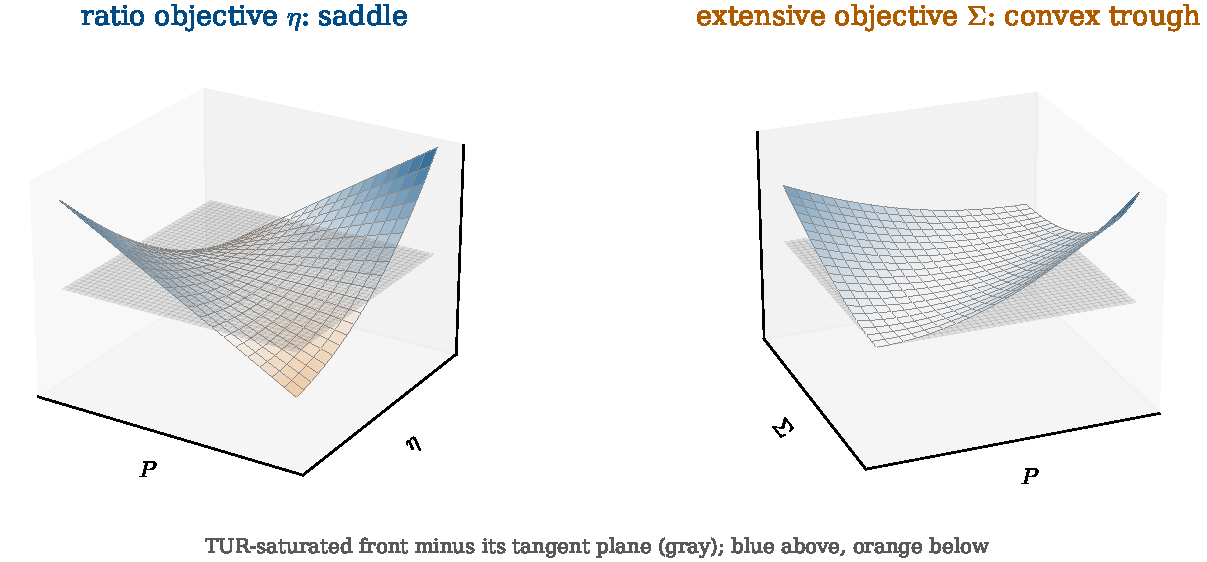
\includegraphics[width=\linewidth]{figs/fig0_saddle.pdf}
\caption{The same TUR-saturating front of Sec.~\ref{sec:case}, minus its tangent plane at an interior
point, in the ratio formulation (left: saddle, Theorem~\ref{thm:saddle}) and the extensive formulation
(right: convex and flat along a ray, Theorem~\ref{thm:perspective} and Corollary~\ref{cor:degenerate}).
Axes are rescaled; the sign of the curvature is invariant under rescaling.}
\label{fig:saddle}
\end{figure}

%=====================================================================
\section{Diagnostics}
\label{sec:diagnostics}
%=====================================================================

\subsection{Support test}
For a sampled front $\mathcal{F}$ and a point $p$ we solve the linear program
\begin{equation}
s^*(p) = \min_{w \ge 0,\ \sum w_i = 1}\ \max_{q \in \mathcal{F}}\ w\cdot(p - q),
\label{eq:gap}
\end{equation}
i.e., minimize $s$ subject to $w\cdot(p-q) \le s$ for all $q$. Then $s^* = 0$ if and only if $p$ is
supported, and $s^* > 0$ is its distance from being reachable in normalized units. We declare $p$
unsupported when $s^* > 10^{-3}$ in coordinates normalized to the unit cube.

\subsection{Hypervolume ceiling and loss decomposition}
The HV of the supported subset of a reference front is an upper bound on the HV of the solutions
that \emph{any} weighted-sum method can return, whatever its weights. We call it the
\emph{weighted-sum ceiling} and split the HV loss of a weighted-sum method into
\begin{align}
\text{reachability loss} &= \mathrm{HV}(\text{reference}) - \text{ceiling},\\
\text{distribution loss} &= \text{ceiling} - \mathrm{HV}(\text{method}).
\end{align}
The first cannot be recovered by any choice of weights; the second can, in principle, by better
weights.

\subsection{Multiplicative loss of the best reachable solution}
For a point $p$ of the front in the original (physically meaningful) objectives and the set $S$ of
supported solutions, let
\begin{equation}
\varepsilon(p) = \min_{s\in S}\ \max_i\ \rho_i(p,s) - 1,
\end{equation}
with $\rho_i = p_i/s_i$ for maximized and $s_i/p_i$ for minimized positive objectives. This is the
multiplicative $\varepsilon$-indicator~\cite{Zitzler2003} of $S$ with respect to $\{p\}$: the best
solution a weighted-sum designer can obtain is at least a fraction $\varepsilon$ worse than $p$ in some
objective.

%=====================================================================
\section{Case study: a finite-time quantum Otto engine}
\label{sec:case}
%=====================================================================

\subsection{Model}
The working medium is a two-level system (qubit) with energy gap $\omega$ ($\hbar = k_B = 1$),
as in the device proposed (as a refrigerator) in Ref.~\cite{Karimi2016}: a flux-tunable
superconducting qubit coupled to two resonators terminated by resistors at different temperatures. The Otto cycle alternates (i) contact with a hot bath at
$T_h$ with gap $\omega_h$ for a time $\tau_h$, (ii) a fast change of the gap to $\omega_c$, (iii)
contact with a cold bath at $T_c$ for $\tau_c$, and (iv) a fast change back. During contact the
excited-state probability relaxes as $p \to a + (p-a)e^{-\gamma\tau}$ toward the Gibbs value
$a = 1/(1+e^{\omega/T})$. Heat is exchanged when the population changes at fixed gap and work when
the gap changes at fixed population. The stochastic work per cycle is
$w = (\omega_h - \omega_c)(s_1 - s_2)$, with $s_1, s_2 \in \{0,1\}$ the qubit state at the two gap
changes.

Mean power $P$ and power fluctuations $\Delta P = \lim_t \operatorname{Var}(W_t)/t$ follow exactly
from the largest eigenvalue of a $2\times2$ tilted transfer matrix of one cycle (full counting
statistics), in closed form, and were validated against Monte Carlo simulation. The efficiency is
$\eta = 1 - \omega_c/\omega_h$ and the entropy production rate is
$\Sigma = P(\etaC - \eta)/(\eta T_c)$, with $\etaC = 1 - T_c/T_h$. We use $T_h = 1$, $T_c = 0.5$,
$\gamma = 1$, gap-change duration $0.05$ and four decision variables:
$\omega_h \in [0.1,10]$, $\omega_c/\omega_h \in [T_c/T_h, 1]$ and
$\log_{10}\tau_{h,c} \in [-2,1]$. Each evaluation is a closed-form expression.

\subsection{Why the structure is exact}
Thermodynamics bounds the precision of the engine through the thermodynamic uncertainty relation
(TUR)~\cite{Barato2015,Gingrich2016,Pietzonka2018}, $\Delta P\,\Sigma \ge 2P^2$. On the Pareto front of
this engine the bound is saturated (median ratio $\xi = 2P^2/(\Delta P\,\Sigma) = 0.996$, maximum
$1.005$; cyclic engines may exceed $1$ slightly~\cite{Holubec2018}), in line with earlier
observations for fast Otto cycles~\cite{Erdman2023}. Saturation gives
\begin{equation}
\Delta P = P\,\varphi(\eta), \qquad \varphi(\eta) = \frac{2T_c\,\eta}{\etaC - \eta},
\end{equation}
a product structure with $a = P$, $r = \eta$, $c = \Delta P$. Entropy production is the extensive
reformulation: $\Sigma = P\,s(\eta)$ with $s(\eta) = (\etaC - \eta)/(\eta T_c)$ decreasing, and
$\chi(u) = \varphi(s^{-1}(u)) = 2/u$, which is convex. Hence $\Delta P = 2P^2/\Sigma$. The two
formulations used in the experiments are
\begin{align}
\text{ratio:}\quad & f = (-P,\ -\eta,\ \Delta P),\\
\text{extensive:}\quad & f = (-P,\ \Delta P,\ \Sigma).
\end{align}
Theorems~\ref{thm:saddle} and~\ref{thm:perspective} predict a saddle in the first and a convex,
ray-degenerate front in the second. The extensive formulation is the one used by Erdman
\emph{et al.}~\cite{Erdman2023} in their weighted figure of merit.

\subsection{A variant that breaks the structure}
To test what happens when the product structure fails, we use the quantum-dot engine of
Ref.~\cite{Erdman2023} with piecewise control: the cycle is split into 8 steps, each with its own gap
and bath, plus the cycle duration (17 variables). Free control lets the cycle violate the stationary
TUR, so the front is no longer product-structured.

\subsection{A degenerate limit}
\label{sec:lr}
Near equilibrium (linear response), the exact fronts of Almanza-Marrero
\emph{et al.}~\cite{Almanza2026} collapse to a one-parameter curve on the TUR surface,
$P = 4P_{\max}\bar\eta(1 - \bar\eta)$ with $\bar\eta = \eta/\etaC$, because power and efficiency are
locked by a single effective degree of freedom. That curve lies on the saddle but is fully supported
(Remark 1).

%=====================================================================
\section{Experimental setup}
\label{sec:setup}
%=====================================================================

\paragraph*{Algorithms} NSGA-II~\cite{Deb2002}, NSGA-III~\cite{DebJain2014},
SMS-EMOA~\cite{Beume2007}, RVEA~\cite{Cheng2016} (pymoo 0.6.2~\cite{Blank2020}); MOEA/D with
normalized Tchebycheff~\cite{ZhangLi2007}; MOEA/D-AWA~\cite{Qi2014}; and MOEA/D-WS, identical to
MOEA/D but with the weighted-sum scalarization, which is the evolutionary counterpart of sweeping the
weights of a linear figure of merit. All use $N = 105$ (Das--Dennis weights, 13 divisions), SBX
(probability 1, $\eta_c = 20$) and polynomial mutation ($\eta_m = 20$). MOEA/D variants use a
neighborhood of $10\%$ of $N$, $\delta = 0.9$, $n_r = 2$ and online normalization. MOEA/D-AWA follows
Ref.~\cite{Qi2014}: WS-transformed weights, an external population of $1.5N$ truncated by sparsity,
and replacement of $5\%$ of the weights every 10 generations after $80\%$ of the run.

\paragraph*{Budgets} 400 generations ($42\,000$ evaluations) on the Otto engine and 3000 generations
($315\,000$) on the piecewise model; 30 independent runs per algorithm and formulation.

\paragraph*{Reference fronts} Nondominated union of all runs plus a dense grid of the four variables
(Otto) or five long SMS-EMOA runs (piecewise), thinned on a $60^3$ voxel grid (about 4\,600--4\,900
points for Otto and 2\,100--2\,400 for the piecewise model).

\paragraph*{Metrics and statistics} HV with reference point $1.1$ in coordinates normalized by the
reference front~\cite{Zitzler1999}; IGD+~\cite{Ishibuchi2015}. Each algorithm is compared with
MOEA/D-AWA by a two-sided Mann--Whitney test~\cite{MannWhitney1947} with Holm
correction~\cite{Holm1979} over six comparisons.

%=====================================================================
\section{Results}
\label{sec:results}
%=====================================================================

\subsection{Synthetic product-structured fronts}

Table~\ref{tab:synthetic} applies the support test to synthetic fronts with
$D = \{0 < a \le 4r(1-r)\}$, extensive cost $b = a(1/r - 1)$, and four profiles $\varphi$ (1600
points each). In the ratio formulation 86--93\% of the points are unsupported for every $\varphi$, as
Theorem~\ref{thm:saddle} predicts. In the extensive formulation none are, except for the profile
chosen so that $\chi$ is concave, where 78\% remain unsupported: the reformulation helps exactly when
$\chi$ is convex (Theorem~\ref{thm:perspective}).

\begin{table}[t]
\caption{Unsupported fraction (max gap) of synthetic product-structured fronts.}
\label{tab:synthetic}
\centering
\footnotesize
\begin{tabular}{lcc}
\toprule
$\varphi(r)$ & ratio $(a, r, c)$ & extensive $(a, b, c)$\\
\midrule
$2r/(1-r)$ (TUR-like), $\chi$ convex & 86\% (0.081) & 0\% (0)\\
$r$, $\chi$ convex & 92\% (0.090) & 0\% (0)\\
$e^{2r}$, $\chi$ convex & 90\% (0.081) & 0\% (0)\\
$6 - 1/(2r^2)$, $\chi$ concave & 93\% (0.188) & 78\% (0.026)\\
\bottomrule
\end{tabular}
\end{table}

\subsection{Otto engine: geometry and algorithms}

On the reference front, 91\% of the points are unsupported in the ratio formulation, with gaps up to
$0.077$; in the extensive formulation only 4\%, with gaps below $0.005$. The residual 4\% may reflect a
slightly nonconvex domain $D'$ and the fact that $\xi$ is not exactly 1.

\begin{table}[t]
\caption{Otto engine, 30 runs: median HV (higher is better), median IGD+ and mean number of distinct
solutions. Every difference with respect to MOEA/D-AWA is significant ($p = 1.8\times10^{-10}$, Holm).}
\label{tab:otto}
\centering
\footnotesize
\setlength{\tabcolsep}{3.5pt}
\begin{tabular}{lcccccc}
\toprule
 & \multicolumn{3}{c}{ratio $(P,\eta,\Delta P)$} & \multicolumn{3}{c}{extensive $(P,\Delta P,\Sigma)$}\\
 & HV & IGD+ & dist. & HV & IGD+ & dist.\\
\midrule
SMS-EMOA & \textbf{1.0425} & 0.0276 & 105 & \textbf{1.1868} & 0.0183 & 104\\
MOEA/D-AWA & 1.0404 & \textbf{0.0198} & 105 & 1.1829 & \textbf{0.0142} & 105\\
MOEA/D & 1.0385 & 0.0251 & 94 & 1.1744 & 0.0220 & 94\\
NSGA-III & 1.0310 & 0.0252 & 104 & 1.1700 & 0.0227 & 104\\
RVEA & 1.0269 & 0.0277 & 89 & 1.1683 & 0.0224 & 87\\
NSGA-II & 1.0073 & 0.0380 & 104 & 1.1612 & 0.0275 & 104\\
MOEA/D-WS & 0.9670 & 0.0745 & 63 & 1.1220 & 0.0664 & 68\\
\midrule
reference front & 1.0810 & & & 1.2114 & &\\
WS ceiling & \textbf{0.9950} & & & 1.2113 & &\\
WS loss: reach.\ + distr. & \multicolumn{3}{c}{$\mathbf{0.086} + 0.028$} & \multicolumn{3}{c}{$0.0001 + \mathbf{0.089}$}\\
\bottomrule
\end{tabular}
\end{table}

Table~\ref{tab:otto} and Fig.~\ref{fig:hv} show that MOEA/D-WS is last in both formulations and loses a
similar amount of HV, but for different reasons, as the theory predicts. In the ratio formulation
most of the loss is reachability: no weight vector can recover it, and six of the seven algorithms,
including NSGA-II, exceed the ceiling of any weighted-sum method. In the extensive formulation the
ceiling coincides with the reference front and the whole loss is distribution: MOEA/D-WS returns only
68 distinct solutions out of 105, the crowding predicted by Corollary~\ref{cor:degenerate}. Among the
other algorithms, SMS-EMOA attains the best HV and MOEA/D-AWA the best IGD+ in both formulations, and
adaptive weights improve on fixed Tchebycheff weights.

\begin{figure*}[t]
\centering
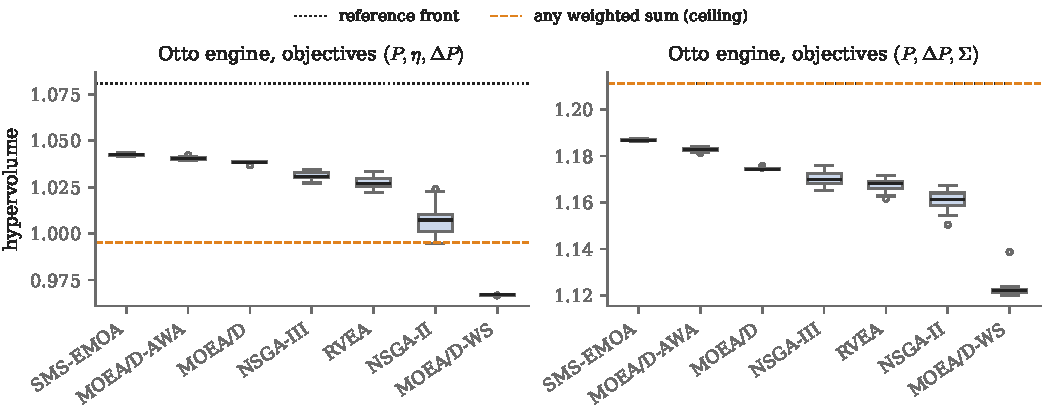
\includegraphics[width=0.85\linewidth]{figs/fig3_hv_otto.pdf}
\caption{HV of seven MOEAs on the Otto engine (30 runs). Dotted: reference front. Dashed: ceiling of
any weighted-sum method. In the ratio formulation (left) the ceiling lies below six algorithms; in
the extensive formulation (right) it coincides with the reference front.}
\label{fig:hv}
\end{figure*}

\subsection{Otto engine: what a weighted-sum designer loses}

Fig.~\ref{fig:cost} maps the multiplicative loss $\varepsilon$ over the front in the original
objectives $(P,\eta,\Delta P)$. A weighted sum in the ratio formulation reaches 11\% of the front; for
the rest, the best reachable solution is worse by a median of 14\% in some objective, and 60\% of the
front has $\varepsilon > 10\%$. The losses concentrate in the low-power, high-efficiency region. A
weighted sum in the extensive formulation, evaluated on the same solutions, reaches 98\% of its front,
and its median loss over the ratio front is 0\% (7\% of the front has $\varepsilon > 5\%$).

\begin{figure*}[t]
\centering
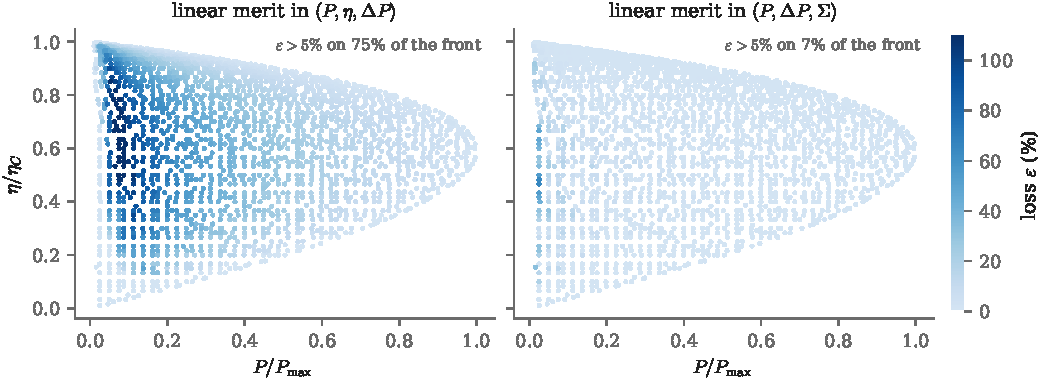
\includegraphics[width=0.85\linewidth]{figs/fig2_cost.pdf}
\caption{Loss $\varepsilon$ of the best solution reachable by a weighted sum, over the Otto front
in the $(P,\eta)$ plane. Left: weighted sum in the ratio formulation. Right: in the extensive
formulation.}
\label{fig:cost}
\end{figure*}

\subsection{Degenerate limit}

For the linear-response model of Ref.~\cite{Almanza2026} we sampled $2\times10^5$ random designs: the
nondominated designs follow the analytic curve to within $2\times10^{-5}$, saturate the TUR to within
$10^{-5}$, and the support test finds no unsupported point in any combination of three or four of its
objectives. A weighted sum that includes the ratio $\eta$ is therefore exact there, in agreement with
Remark 1. Fig.~\ref{fig:lr} contrasts the curve with the two-dimensional front of the Otto engine.

\begin{figure}[t]
\centering
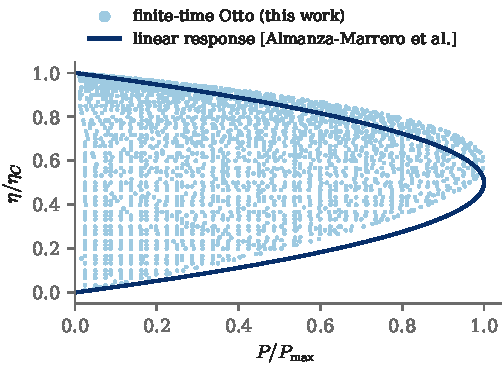
\includegraphics[width=\linewidth]{figs/fig4_linear_response.pdf}
\caption{Otto front projected on $(P,\eta)$ (points; two-dimensional) and the linear-response front
(curve; one-dimensional), each normalized by its own maximum power.}
\label{fig:lr}
\end{figure}

\subsection{Breaking the structure: piecewise control}

In the 17-variable model the front violates the stationary TUR ($\xi$ up to $4.0$; 81\% of the
reference front has $\xi > 1$), so neither theorem applies. The support test flags 31\%
(extensive) and 48\% (ratio) of the reference front at tolerance $10^{-3}$, but the gaps are small
(median about $0.003$; below 1\% of points exceed $10^{-2}$) and the weighted-sum ceiling is within
0.1\% and 0.2\% of the reference HV (Table~\ref{tab:pw}, Fig.~\ref{fig:pw}). The front is nearly
convex in both formulations. MOEA/D-WS still differs between formulations, ranking second in the
extensive one and behind MOEA/D-AWA in the ratio one, but its loss is now distribution only, which
the theory does not address. MOEA/D-AWA and fixed-weight Tchebycheff MOEA/D are statistically
indistinguishable on this problem ($p = 0.71$ and $0.49$).

\begin{table}[t]
\caption{Piecewise model, 30 runs, median HV; $p$-values (Holm) vs.\ MOEA/D-AWA.}
\label{tab:pw}
\centering
\footnotesize
\begin{tabular}{lcc}
\toprule
 & ratio $(P,\eta,\Delta P)$ & extensive $(P,\Delta P,\Sigma)$\\
\midrule
SMS-EMOA & 1.0846 ($5\times10^{-8}$) & 1.2094 ($3\times10^{-10}$)\\
MOEA/D-AWA & 1.0654 & 1.1867\\
MOEA/D & 1.0600 (0.49) & 1.1876 (0.71)\\
NSGA-III & 1.0604 (0.030) & 1.1844 (0.41)\\
MOEA/D-WS & 1.0586 (0.017) & 1.1929 (0.011)\\
RVEA & 0.9989 ($2\times10^{-9}$) & 1.1658 ($2\times10^{-5}$)\\
NSGA-II & 1.0009 ($2\times10^{-10}$) & 1.1337 ($3\times10^{-10}$)\\
\midrule
reference / WS ceiling & 1.1208 / 1.1184 & 1.2284 / 1.2276\\
WS loss: reach.\ + distr. & $0.0024 + 0.060$ & $0.0008 + 0.035$\\
\bottomrule
\end{tabular}
\end{table}

\begin{figure*}[t]
\centering
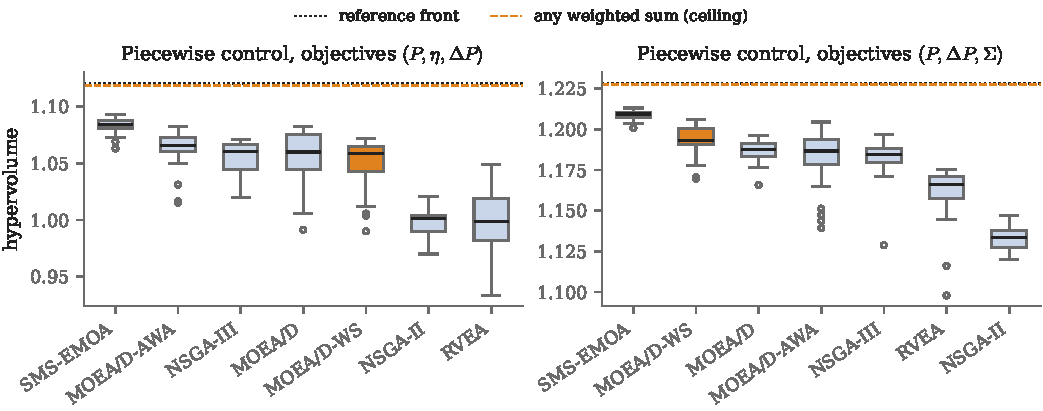
\includegraphics[width=0.85\linewidth]{figs/fig5_hv_piecewise.pdf}
\caption{HV of seven MOEAs on the piecewise model (30 runs). Lines as in Fig.~\ref{fig:hv}. The
weighted-sum ceiling is close to the reference front in both formulations.}
\label{fig:pw}
\end{figure*}

%=====================================================================
\section{Discussion}
\label{sec:discussion}
%=====================================================================

\paragraph*{Guidelines} (i) Before trusting a weighted-sum sweep, run the support test of
Eq.~\eqref{eq:gap} on a front obtained by a dominance-based or Tchebycheff method; it costs one small
linear program per point. (ii) When a ratio objective appears together with an extensive output and a
cost proportional to it, rewrite the ratio as an extensive cost and check that the profile $\chi$ is
convex; if it is, every solution becomes reachable. (iii) Even then, weighted-sum decomposition loses
quality through degeneracy along rays; Tchebycheff, adaptive weights or indicator-based selection
avoid both losses. (iv) Report the weighted-sum ceiling alongside HV when comparing scalarizations; it
separates what the weights could fix from what they cannot.

\paragraph*{A benchmark with controllable geometry} The Otto engine offers two formulations of the same
solutions with known front shapes (saddle and ray-degenerate convex), exact and cheap evaluations,
four variables and a physical interpretation. Its piecewise variant offers a harder, higher-dimensional
problem with a nearly convex front. Both complement synthetic suites~\cite{Deb2005DTLZ} and existing
real-world suites~\cite{Tanabe2020}.

\paragraph*{Limitations} The theorems assume an exact product structure; real fronts satisfy it only
approximately, and the piecewise model shows that the effect vanishes when the structure is broken
strongly. How the reachability loss interpolates between these regimes is open. The support test and
the ceiling use a discrete reference front, so they carry an error of the order of the tolerance.
Adaptive weights gave a clear advantage on the Otto engine but none on the piecewise model.

%=====================================================================
\section{Conclusion}
%=====================================================================

Whether a weighted-sum decomposition can reach a Pareto front is not only a property of the problem
but also of the objectives chosen to describe it. For fronts in which a cost is proportional to an
extensive output at fixed ratio, the ratio formulation produces a saddle that hides every interior
solution from any weighted sum, and an extensive reformulation produces a convex, ray-degenerate front
when a one-dimensional profile is convex. The proposed diagnostics separate the resulting
reachability loss from the distribution loss caused by degeneracy, and a quantum heat engine provides
an exact real-world instance of both effects.

\section*{Data and code availability}
Code, raw runs and analysis scripts are available at \url{https://github.com/uwo-o/hidden-front}. All results can be reproduced with the scripts in that repository.

\appendices
\section{Implementation checks}
Our MOEA/D implementation was checked on DTLZ2 (regular front) and DTLZ7 (disconnected
front)~\cite{Deb2005DTLZ} with three objectives, $N = 105$, 300 generations and 10 runs per variant
(Table~\ref{tab:dtlz}). The WS-transformation of the weights~\cite{Qi2014} and the adaptive weight
adjustment each lower IGD+, and the adjustment period used in the main experiments (10 generations)
is the best of the two tested. On DTLZ7, one or two runs of every variant miss a disconnected region
(IGD+ $\approx 0.66$).

\begin{table}[h]
\caption{Median IGD+ on DTLZ benchmarks (10 runs). All variants use Tchebycheff scalarization.}
\setlength{\tabcolsep}{3pt}
\label{tab:dtlz}
\centering
\footnotesize
\begin{tabular}{lcccc}
\toprule
 & MOEA/D & +WS-tr. & AWA, $w_{ag}{=}20$ & AWA, $w_{ag}{=}10$\\
\midrule
DTLZ2 & 0.0344 & 0.0231 & 0.0210 & \textbf{0.0207}\\
DTLZ7 & 0.0445 & 0.0346 & 0.0338 & \textbf{0.0319}\\
\bottomrule
\end{tabular}
\end{table}

The engine statistics were checked against Monte Carlo simulation
of the jump process and against finite differences of the cumulant generating function; the
piecewise model reproduces the four-variable engine to $10^{-9}$ when restricted to it.

\bibliographystyle{IEEEtran}
\bibliography{refs}

\end{document}
